\chapter{Неопределенный интеграл}
\label{cha:Indefinite_Integral}

\section{Первообразная и неопределенный интеграл}
\label{sec:Antiderivative_and_Indefinite_Integral}

\subsection{Первообразная}
\label{sub:antiderivative}

$ f, F: \ X \longrightarrow \bbR, \ X = \left( a;b \right) $

\dfn{Первообразная}{
  \label{dfn:Anitderivative}
  \textbf{Первообразной функцией} функции $f$ на $X$ называется функция $F$, для которой справедливо: \[
    \left( F \text{ --- дифф. на } X \right) \ \wedge \ \left( F'(x) = f(x) \right) 
  .\]
}

\ex{}{
  \label{example:Antiderivative_x_Cubed}
  \[
    \text{Пусть } f(x) = x^3, \text{ тогда } F(x) = \frac{x^{4}}{4}, \ F(x) = \frac{x^{4}}{4} + 2, \ F(x) = \frac{x^{4}}{4} - 2, \ F(x) = \frac{x^{4}}{4} - 5
  .\] 

  \begin{figure}[H]
  \centering
  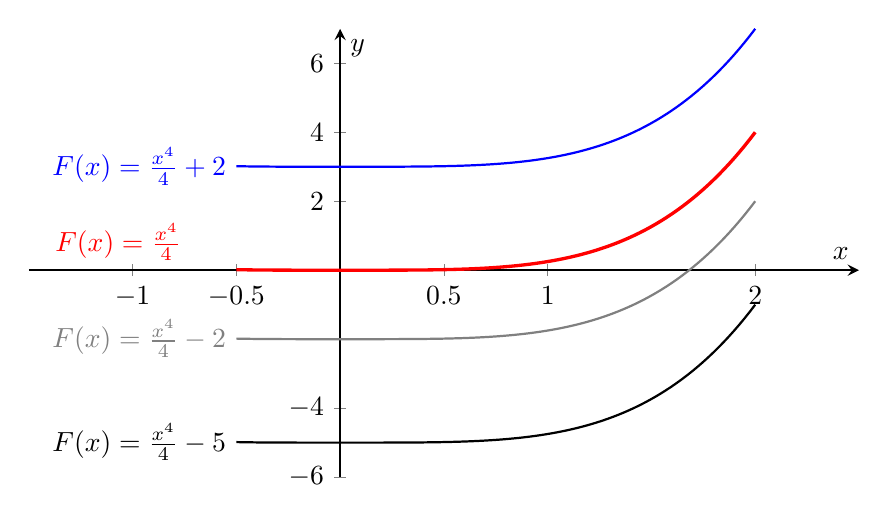
\begin{tikzpicture}
    \begin{axis}[
      width = \textwidth,
      height=\axisdefaultheight,
      xmin = -1.5, xmax = 2.5, ymin = -6, ymax = 7,
      axis lines = middle,
      xlabel = $x$,
      ylabel = $y$,
      samples = 100,
      thick,
      xtick = {-1, -.5, .5, 1, 2},
      ytick = {-6, -4, 2, 4, 6}
      ]
      \addplot[very thick, domain=-.5:2, color=red]{x^4/4} node[xshift=-16pt, yshift=10pt, left, pos=0]{$F(x) = \frac{x^{4}}{4}$};
      \addplot[domain=-.5:2, color=blue]{x^4/4 + 3} node[left, pos=0]{$F(x) = \frac{x^{4}}{4} + 2$};
      \addplot[domain=-.5:2, color=gray]{x^4/4 - 2} node[left,pos=0]{$F(x) = \frac{x^{4}}{4} - 2$};
      \addplot[domain=-.5:2, color=black]{x^4/4 - 5} node[left,pos=0]{$F(x) = \frac{x^{4}}{4} - 5$};
    \end{axis}
  \end{tikzpicture}
  \caption{Графики некоторых первообразных функции $x^3$}
  \label{tikzplot:Antiderivative_x_Cubed}
\end{figure}

}

\nt{
  Опираясь на пример \ref{example:Antiderivative_x_Cubed} нетрудно заметить, что
  \[
    F(x) \text{ --- первообр. $f$ на $X$} \xLeftrightarrow{\text{def}} F'(x) = f(x) \ \forall x \in X \Rightarrow F(x) + C \text{ --- первообр. $f$ на $X$}, \ C = \text{const} 
  .\] 
}

\thm{Отличие первообразных на постоянную}{
  Любые две первообразные функции $f$ отличаются на постоянную:
  \[
   F_1, F_2 \text{ --- первообразн. $f$ на $X$}
  \]
  \[
  \Updownarrow
  \] 
  \[
    F_1(x) = F_2(x)+C, \ C = \text{const}
  .\]
  \textbf{Доказательство:}
  \[
  \begin{array}{lcl}
    F_1 \text{ --- первообр. $f$ на $x$} & \xLeftrightarrow{\text{def}} & F_1'(x) = f(x) \  \forall x \in X \\
    F_2 \text{ --- первообр. $f$ на $x$} & \xLeftrightarrow{\text{def}} & F_2'(x) = f(x) \ \forall x \in X
  \end{array}  
  %FIXME!  Add reference to LAGRANGE THEOREM
  \Rightarrow F_1' = F_2' \ \forall x \in X \xRightarrow{FIXME! \ref{example:Antiderivative_x_Cubed}} F_2 - F_1 = C
  .\] 
}

\nt{
  Первообразная зависит от множества, на котором мы её рассматриваем.
}

\dfn{Обобщенная первообразная}{
  \label{dfn:Generalized_Antiderivative}
  \textbf{Обобщенной первообразной} $F(x)$ функции $f(x)$ на множестве $X$ называется функция, удовлетворяющая условиям:
  \begin{enumerate}
    \item $F \in C^{1}(X)$
    \item $F$ --- дифф. на $X \setminus A$, где $A$ --- конечное множество
    \item $F'(x) = f(x)$
  \end{enumerate}
}



\subsection{Неопределенный интеграл}
\label{sub:Indefinite_Integral}

\dfn{Неопределенный интеграл}{
  \label{dfn:Indefinite_Integral}
\textbf{Неопределенным интегралом} от $f(x)$ на $X$ называется класс всех первообразных функции $f(x)$ на $X$, т. е. множество $\{ F(x) + C \}, \ C = \text{const}$. Неопределенный интеграл обозначается
  \[
    \int f(x) dx = F(x) + C  \text{, где }
  \] 
  \begin{itemize}[label={}]
    %\item $C$ --- const,
    \item $\int$ --- знак интеграла,
    \item $f(x)$ ---  подинтегральная функция,
    \item $f(x)dx$ --- подинтегральное выражение,
    \item $dx$ ---  дифференциал независимой переменной.
  \end{itemize}
}

\ex{Интегралы от простых функций}{
  \label{ex:Examples_of_Integration}
  
  \begin{itemize}[label={}]
    \item $ \int e^{x} dx = e^{x} + C $
    \item $ \int x^{3} dx = \frac{x^{4}}{4} + C $
    \item $ \int \frac{1}{1+x^2} dx = \arctg x + C $
  \end{itemize}
}

\pagebreak
\textbf{Свойства неопределенного интеграла:}
\label{prop:Indefinite_Integral}
\begin{enumerate}[label=\bfseries\tiny\protect\circled{\small\arabic*}]
  \item Дифференциал от интеграла есть подинтегральное выражение: 
  \[
      \left( \int F'(x) dx \right)'= f(x) \ \wedge \ d \left( \int f(x)dx \right) = dx
  .\] 
  \textbf{Доказательство:}
  \[
    \int f(x) dx = F(x) + C \Rightarrow \left( \int f(x) dx \right)' = \left( F(x) + C \right)' = F'(x) + C' = f(x)
  .\]
  \item Интеграл от производной функции равен самой функции:
    \[
    \int F'(x) dx = \int dF(x) = F(x) + C
    .\] 
    \textbf{Доказательство:} следует из определения неопределенного интеграла \ref{dfn:Indefinite_Integral} и первообразной \ref{dfn:Anitderivative}.

  \item Интеграл от линейной комбинации функций равен линейной комбинайии интегралов от функций: 
    \[
    \exists \int f_1(x) dx, \ \exists \int f_2(x) dx, \ \forall \alpha, \beta \in \bbR \Rightarrow \exists \int \left( \alpha f_1(x) + \beta f_2(x)  \right) dx = \alpha \int f_1(x) dx + \beta \int f_2(x) dx 
    .\] 
    \textbf{Доказательство:}
    \[
     \left(  \alpha \int f_1(x) dx + \beta \int f_2(x) dx \right)' = \alpha \left( \int f_1(x)dx \right)' \left( \int f_2(x)dx \right)' = \alpha f_1(x) + \beta f_2(x)
    .\] 
    \[
    \Downarrow
    \] 
    \[
      \left(  \alpha \int f_1(x) dx + \beta \int f_2(x) dx \right) \text{ --- первообразная функции } \alpha f_1(x) + \beta f_2(x)
    .\] 
\end{enumerate}



\subsection{Таблица основных интегралов}%
\label{sub:Table_of_Integrals}

\begin{multicols}{2}
\begin{enumerate}
  \item $\int x^{\alpha} = \frac{x^{\alpha+1}}{\alpha +1} + C, \ \alpha \neq -1$
  \item $\int \frac{1}{x}dx = \ln |x| + C$
  \item $\int a^{x} dx = \frac{a^x}{\ln a} + C, \ 0<a\neq 1$
  \item $\int \cos x dx = \sin x + C$
  \item $\int \sin x dx = -\cos x + C$
  \item $\int \sh x dx = \ch x + C$
  \item $\int \ch x dx = \sh x + C$
  \item $\int \frac{1}{\cos^2x} dx = \tg x + C$
  \item $\int \frac{1}{\sin^2x} dx = -\ctg x + C$
  \item $\int \frac{1}{\ch^2x} dx = \th x + C$
  \item $\int \frac{1}{\sh^2x} dx = -\cth x + C$
  \item $\int \frac{dx}{1+x^2} = \arctg x + C \ (- \arcctg x + C)$
  \item $\int \frac{dx}{\sqrt{1-x^2}} = \arcsin x + C \ (- \arccos x + C)$
  \item $\int \frac{dx}{x^2-a^2} = \frac{1}{2a} \ln \left| \frac{x-a}{x+a} \right| + C $
  \item $\int \frac{dx}{\sqrt{x^2 \pm a^2}} = \ln \left| x + \sqrt{x^2 \pm a^2} \right|$

\end{enumerate}
\end{multicols}

